\documentclass[1p]{elsarticle_modified}
%\bibliographystyle{elsarticle-num}

%\usepackage[colorlinks]{hyperref}
%\usepackage{abbrmath_seonhwa} %\Abb, \Ascr, \Acal ,\Abf, \Afrak
\usepackage{amsfonts}
\usepackage{amssymb}
\usepackage{amsmath}
\usepackage{amsthm}
\usepackage{scalefnt}
\usepackage{amsbsy}
\usepackage{kotex}
\usepackage{caption}
\usepackage{subfig}
\usepackage{color}
\usepackage{graphicx}
\usepackage{xcolor} %% white, black, red, green, blue, cyan, magenta, yellow
\usepackage{float}
\usepackage{setspace}
\usepackage{hyperref}

\usepackage{tikz}
\usetikzlibrary{arrows}

\usepackage{multirow}
\usepackage{array} % fixed length table
\usepackage{hhline}

%%%%%%%%%%%%%%%%%%%%%
\makeatletter
\renewcommand*\env@matrix[1][\arraystretch]{%
	\edef\arraystretch{#1}%
	\hskip -\arraycolsep
	\let\@ifnextchar\new@ifnextchar
	\array{*\c@MaxMatrixCols c}}
\makeatother %https://tex.stackexchange.com/questions/14071/how-can-i-increase-the-line-spacing-in-a-matrix
%%%%%%%%%%%%%%%

\usepackage[normalem]{ulem}

\newcommand{\msout}[1]{\ifmmode\text{\sout{\ensuremath{#1}}}\else\sout{#1}\fi}
%SOURCE: \msout is \stkout macro in https://tex.stackexchange.com/questions/20609/strikeout-in-math-mode

\newcommand{\cancel}[1]{
	\ifmmode
	{\color{red}\msout{#1}}
	\else
	{\color{red}\sout{#1}}
	\fi
}

\newcommand{\add}[1]{
	{\color{blue}\uwave{#1}}
}

\newcommand{\replace}[2]{
	\ifmmode
	{\color{red}\msout{#1}}{\color{blue}\uwave{#2}}
	\else
	{\color{red}\sout{#1}}{\color{blue}\uwave{#2}}
	\fi
}

\newcommand{\Sol}{\mathcal{S}} %segment
\newcommand{\D}{D} %diagram
\newcommand{\A}{\mathcal{A}} %arc


%%%%%%%%%%%%%%%%%%%%%%%%%%%%%5 test

\def\sl{\operatorname{\textup{SL}}(2,\Cbb)}
\def\psl{\operatorname{\textup{PSL}}(2,\Cbb)}
\def\quan{\mkern 1mu \triangleright \mkern 1mu}

\theoremstyle{definition}
\newtheorem{thm}{Theorem}[section]
\newtheorem{prop}[thm]{Proposition}
\newtheorem{lem}[thm]{Lemma}
\newtheorem{ques}[thm]{Question}
\newtheorem{cor}[thm]{Corollary}
\newtheorem{defn}[thm]{Definition}
\newtheorem{exam}[thm]{Example}
\newtheorem{rmk}[thm]{Remark}
\newtheorem{alg}[thm]{Algorithm}

\newcommand{\I}{\sqrt{-1}}
\begin{document}

%\begin{frontmatter}
%
%\title{Boundary parabolic representations of knots up to 8 crossings}
%
%%% Group authors per affiliation:
%\author{Yunhi Cho} 
%\address{Department of Mathematics, University of Seoul, Seoul, Korea}
%\ead{yhcho@uos.ac.kr}
%
%
%\author{Seonhwa Kim} %\fnref{s_kim}}
%\address{Center for Geometry and Physics, Institute for Basic Science, Pohang, 37673, Korea}
%\ead{ryeona17@ibs.re.kr}
%
%\author{Hyuk Kim}
%\address{Department of Mathematical Sciences, Seoul National University, Seoul 08826, Korea}
%\ead{hyukkim@snu.ac.kr}
%
%\author{Seokbeom Yoon}
%\address{Department of Mathematical Sciences, Seoul National University, Seoul, 08826,  Korea}
%\ead{sbyoon15@snu.ac.kr}
%
%\begin{abstract}
%We find all boundary parabolic representation of knots up to 8 crossings.
%
%\end{abstract}
%\begin{keyword}
%    \MSC[2010] 57M25 
%\end{keyword}
%
%\end{frontmatter}

%\linenumbers
%\tableofcontents
%
\newcommand\colored[1]{\textcolor{white}{\rule[-0.35ex]{0.8em}{1.4ex}}\kern-0.8em\color{red} #1}%
%\newcommand\colored[1]{\textcolor{white}{ #1}\kern-2.17ex	\textcolor{white}{ #1}\kern-1.81ex	\textcolor{white}{ #1}\kern-2.15ex\color{red}#1	}

{\Large $\underline{10_{47}~(K10a_{15})}$}

\setlength{\tabcolsep}{10pt}
\renewcommand{\arraystretch}{1.6}
\vspace{1cm}\begin{tabular}{m{100pt}>{\centering\arraybackslash}m{274pt}}
\multirow{5}{120pt}{
	\centering
	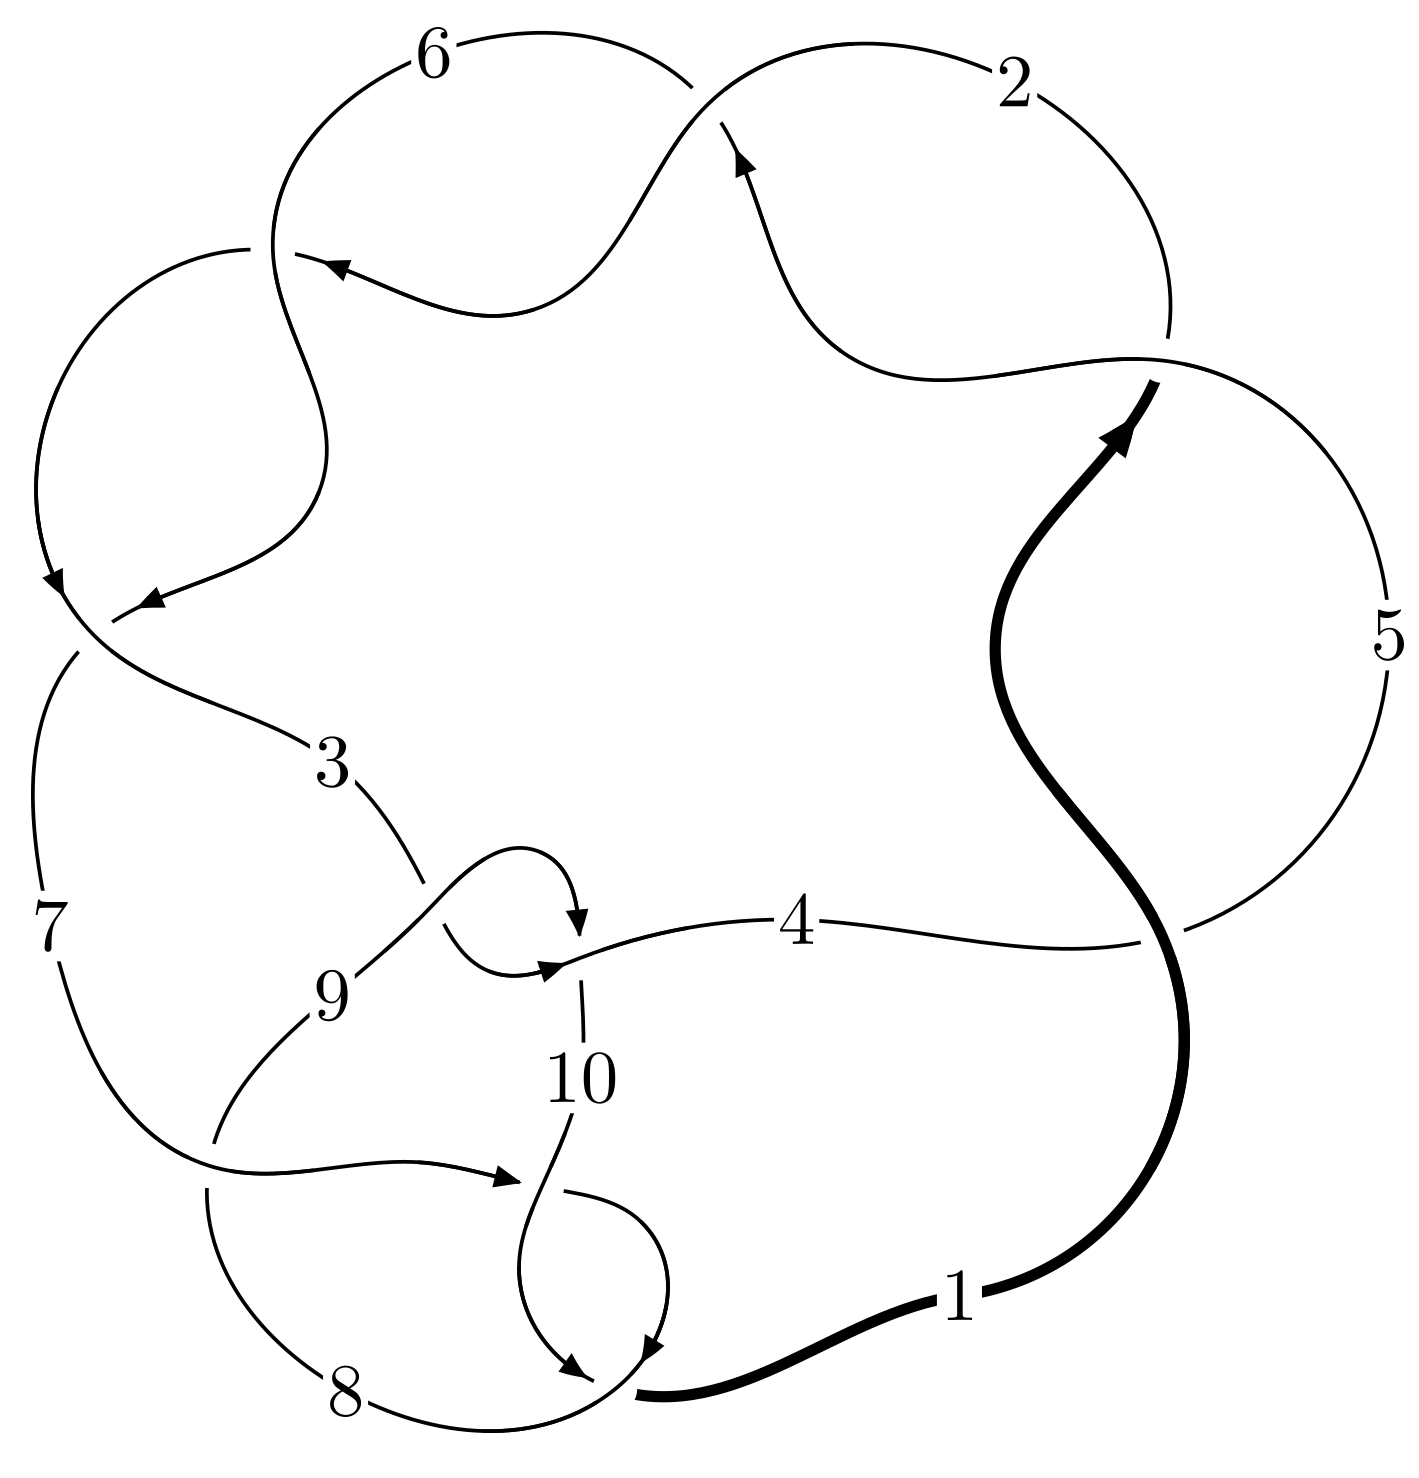
\includegraphics[width=112pt]{../../../GIT/diagram.site/Diagrams/png/131_10_47.png}\\
\ \ \ A knot diagram\footnotemark}&
\allowdisplaybreaks
\textbf{Linearized knot diagam} \\
\cline{2-2}
 &
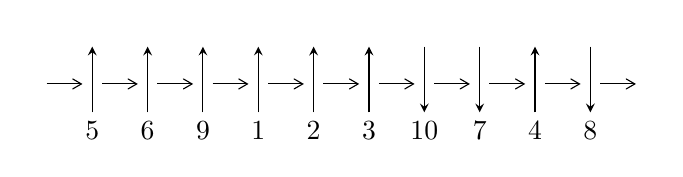
\begin{tikzpicture}[x=20pt, y=17pt]
	% nodes
	\node (C0) at (0, 0) {};
	\node (C1) at (1, 0) {};
	\node (C1U) at (1, +1) {};
	\node (C1D) at (1, -1) {5};

	\node (C2) at (2, 0) {};
	\node (C2U) at (2, +1) {};
	\node (C2D) at (2, -1) {6};

	\node (C3) at (3, 0) {};
	\node (C3U) at (3, +1) {};
	\node (C3D) at (3, -1) {9};

	\node (C4) at (4, 0) {};
	\node (C4U) at (4, +1) {};
	\node (C4D) at (4, -1) {1};

	\node (C5) at (5, 0) {};
	\node (C5U) at (5, +1) {};
	\node (C5D) at (5, -1) {2};

	\node (C6) at (6, 0) {};
	\node (C6U) at (6, +1) {};
	\node (C6D) at (6, -1) {3};

	\node (C7) at (7, 0) {};
	\node (C7U) at (7, +1) {};
	\node (C7D) at (7, -1) {10};

	\node (C8) at (8, 0) {};
	\node (C8U) at (8, +1) {};
	\node (C8D) at (8, -1) {7};

	\node (C9) at (9, 0) {};
	\node (C9U) at (9, +1) {};
	\node (C9D) at (9, -1) {4};

	\node (C10) at (10, 0) {};
	\node (C10U) at (10, +1) {};
	\node (C10D) at (10, -1) {8};
	\node (C11) at (11, 0) {};

	% arrows
	\draw[->,>={angle 60}]
	(C0) edge (C1) (C1) edge (C2) (C2) edge (C3) (C3) edge (C4) (C4) edge (C5) (C5) edge (C6) (C6) edge (C7) (C7) edge (C8) (C8) edge (C9) (C9) edge (C10) (C10) edge (C11) ;	\draw[->,>=stealth]
	(C1D) edge (C1U) (C2D) edge (C2U) (C3D) edge (C3U) (C4D) edge (C4U) (C5D) edge (C5U) (C6D) edge (C6U) (C7U) edge (C7D) (C8U) edge (C8D) (C9D) edge (C9U) (C10U) edge (C10D) ;
	\end{tikzpicture} \\
\hhline{~~} \\& 
\textbf{Solving Sequence} \\ \cline{2-2} 
 &
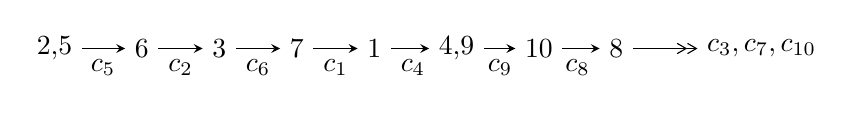
\begin{tikzpicture}[x=28pt, y=7pt]
	% node
	\node (A0) at (-1/8, 0) {2,5};
	\node (A1) at (1, 0) {6};
	\node (A2) at (2, 0) {3};
	\node (A3) at (3, 0) {7};
	\node (A4) at (4, 0) {1};
	\node (A5) at (81/16, 0) {4,9};
	\node (A6) at (49/8, 0) {10};
	\node (A7) at (57/8, 0) {8};
	\node (C1) at (1/2, -1) {$c_{5}$};
	\node (C2) at (3/2, -1) {$c_{2}$};
	\node (C3) at (5/2, -1) {$c_{6}$};
	\node (C4) at (7/2, -1) {$c_{1}$};
	\node (C5) at (9/2, -1) {$c_{4}$};
	\node (C6) at (45/8, -1) {$c_{9}$};
	\node (C7) at (53/8, -1) {$c_{8}$};
	\node (A8) at (9, 0) {$c_{3},c_{7},c_{10}$};

	% edge
	\draw[->,>=stealth]	
	(A0) edge (A1) (A1) edge (A2) (A2) edge (A3) (A3) edge (A4) (A4) edge (A5) (A5) edge (A6) (A6) edge (A7) ;
	\draw[->>,>={angle 60}]	
	(A7) edge (A8);
\end{tikzpicture} \\ 

\end{tabular} \\

\footnotetext{
The image of knot diagram is generated by the software ``\textbf{Draw programme}" developed by Andrew Bartholomew(\url{http://www.layer8.co.uk/maths/draw/index.htm\#Running-draw}), where we modified some parts for our purpose(\url{https://github.com/CATsTAILs/LinksPainter}).
}\phantom \\ \newline 
\centering \textbf{Ideals for irreducible components\footnotemark of $X_{\text{par}}$} 
 
\begin{align*}
I^u_{1}&=\langle 
3 u^{21}-41 u^{19}+\cdots+b-2,\;-2 u^{21}+u^{20}+\cdots+a+1,\;u^{22}-2 u^{21}+\cdots- u+1\rangle \\
I^u_{2}&=\langle 
b- u,\;a-1,\;u^2+u-1\rangle \\
\\
\end{align*}
\raggedright * 2 irreducible components of $\dim_{\mathbb{C}}=0$, with total 24 representations.\\
\footnotetext{All coefficients of polynomials are rational numbers. But the coefficients are sometimes approximated in decimal forms when there is not enough margin.}
\newpage
\renewcommand{\arraystretch}{1}
\centering \section*{I. $I^u_{1}= \langle 3 u^{21}-41 u^{19}+\cdots+b-2,\;-2 u^{21}+u^{20}+\cdots+a+1,\;u^{22}-2 u^{21}+\cdots- u+1 \rangle$}
\flushleft \textbf{(i) Arc colorings}\\
\begin{tabular}{m{7pt} m{180pt} m{7pt} m{180pt} }
\flushright $a_{2}=$&$\begin{pmatrix}0\\u\end{pmatrix}$ \\
\flushright $a_{5}=$&$\begin{pmatrix}1\\0\end{pmatrix}$ \\
\flushright $a_{6}=$&$\begin{pmatrix}1\\- u^2\end{pmatrix}$ \\
\flushright $a_{3}=$&$\begin{pmatrix}u\\- u^3+u\end{pmatrix}$ \\
\flushright $a_{7}=$&$\begin{pmatrix}- u^2+1\\u^4-2 u^2\end{pmatrix}$ \\
\flushright $a_{1}=$&$\begin{pmatrix}- u\\u\end{pmatrix}$ \\
\flushright $a_{4}=$&$\begin{pmatrix}- u^2+1\\u^2\end{pmatrix}$ \\
\flushright $a_{9}=$&$\begin{pmatrix}2 u^{21}- u^{20}+\cdots+4 u-1\\-3 u^{21}+41 u^{19}+\cdots- u+2\end{pmatrix}$ \\
\flushright $a_{10}=$&$\begin{pmatrix}- u^{20}+u^{19}+\cdots-9 u^2+4 u\\- u^{16}+10 u^{14}+\cdots+6 u^3-4 u^2\end{pmatrix}$ \\
\flushright $a_{8}=$&$\begin{pmatrix}u^{21}- u^{20}+\cdots-10 u^2+4 u\\- u^{21}+14 u^{19}+\cdots-3 u^2+1\end{pmatrix}$\\&\end{tabular}
\flushleft \textbf{(ii) Obstruction class $= -1$}\\~\\
\flushleft \textbf{(iii) Cusp Shapes $= -4 u^{21}+5 u^{20}+53 u^{19}-63 u^{18}-292 u^{17}+333 u^{16}+862 u^{15}-974 u^{14}-1448 u^{13}+1758 u^{12}+1295 u^{11}-2051 u^{10}-338 u^9+1521 u^8-426 u^7-628 u^6+422 u^5+65 u^4-139 u^3+35 u^2+14 u+7$}\\~\\
\newpage\renewcommand{\arraystretch}{1}
\flushleft \textbf{(iv) u-Polynomials at the component}\newline \\
\begin{tabular}{m{50pt}|m{274pt}}
Crossings & \hspace{64pt}u-Polynomials at each crossing \\
\hline $$\begin{aligned}c_{1},c_{2},c_{4}\\c_{5},c_{6}\end{aligned}$$&$\begin{aligned}
&u^{22}-2 u^{21}+\cdots- u+1
\end{aligned}$\\
\hline $$\begin{aligned}c_{3},c_{9}\end{aligned}$$&$\begin{aligned}
&u^{22}+u^{21}+\cdots-21 u^2+4
\end{aligned}$\\
\hline $$\begin{aligned}c_{7},c_{10}\end{aligned}$$&$\begin{aligned}
&u^{22}-3 u^{21}+\cdots-8 u+1
\end{aligned}$\\
\hline $$\begin{aligned}c_{8}\end{aligned}$$&$\begin{aligned}
&u^{22}+9 u^{21}+\cdots+40 u+1
\end{aligned}$\\
\hline
\end{tabular}\\~\\
\newpage\renewcommand{\arraystretch}{1}
\flushleft \textbf{(v) Riley Polynomials at the component}\newline \\
\begin{tabular}{m{50pt}|m{274pt}}
Crossings & \hspace{64pt}Riley Polynomials at each crossing \\
\hline $$\begin{aligned}c_{1},c_{2},c_{4}\\c_{5},c_{6}\end{aligned}$$&$\begin{aligned}
&y^{22}-30 y^{21}+\cdots+3 y+1
\end{aligned}$\\
\hline $$\begin{aligned}c_{3},c_{9}\end{aligned}$$&$\begin{aligned}
&y^{22}-15 y^{21}+\cdots-168 y+16
\end{aligned}$\\
\hline $$\begin{aligned}c_{7},c_{10}\end{aligned}$$&$\begin{aligned}
&y^{22}-9 y^{21}+\cdots-40 y+1
\end{aligned}$\\
\hline $$\begin{aligned}c_{8}\end{aligned}$$&$\begin{aligned}
&y^{22}+11 y^{21}+\cdots-1080 y+1
\end{aligned}$\\
\hline
\end{tabular}\\~\\
\newpage\flushleft \textbf{(vi) Complex Volumes and Cusp Shapes}
$$\begin{array}{c|c|c}  
\text{Solutions to }I^u_{1}& \I (\text{vol} + \sqrt{-1}CS) & \text{Cusp shape}\\
 \hline 
\begin{aligned}
u &= \phantom{-}0.964383 + 0.128666 I \\
a &= \phantom{-}0.184838 - 0.945621 I \\
b &= -0.299924 + 0.888159 I\end{aligned}
 & \phantom{-}1.70640 + 2.06027 I & \phantom{-}8.35016 - 3.76643 I \\ \hline\begin{aligned}
u &= \phantom{-}0.964383 - 0.128666 I \\
a &= \phantom{-}0.184838 + 0.945621 I \\
b &= -0.299924 - 0.888159 I\end{aligned}
 & \phantom{-}1.70640 - 2.06027 I & \phantom{-}8.35016 + 3.76643 I \\ \hline\begin{aligned}
u &= -0.889732\phantom{ +0.000000I} \\
a &= \phantom{-}1.34588\phantom{ +0.000000I} \\
b &= \phantom{-}1.19747\phantom{ +0.000000I}\end{aligned}
 & \phantom{-}0.304299\phantom{ +0.000000I} & \phantom{-}11.0200\phantom{ +0.000000I} \\ \hline\begin{aligned}
u &= -1.059960 + 0.353222 I \\
a &= \phantom{-}0.600368 + 0.550351 I \\
b &= \phantom{-}0.830761 + 0.371286 I\end{aligned}
 & \phantom{-}5.17561 - 7.52719 I & \phantom{-}9.40693 + 6.57102 I \\ \hline\begin{aligned}
u &= -1.059960 - 0.353222 I \\
a &= \phantom{-}0.600368 - 0.550351 I \\
b &= \phantom{-}0.830761 - 0.371286 I\end{aligned}
 & \phantom{-}5.17561 + 7.52719 I & \phantom{-}9.40693 - 6.57102 I \\ \hline\begin{aligned}
u &= -1.128070 + 0.227245 I \\
a &= -0.642240 - 0.353090 I \\
b &= -0.804731 - 0.252365 I\end{aligned}
 & \phantom{-}6.69355 - 1.82013 I & \phantom{-}11.99179 + 1.37946 I \\ \hline\begin{aligned}
u &= -1.128070 - 0.227245 I \\
a &= -0.642240 + 0.353090 I \\
b &= -0.804731 + 0.252365 I\end{aligned}
 & \phantom{-}6.69355 + 1.82013 I & \phantom{-}11.99179 - 1.37946 I \\ \hline\begin{aligned}
u &= \phantom{-}0.459979 + 0.506822 I \\
a &= \phantom{-}0.614823 - 0.850759 I \\
b &= -0.713989 + 0.079726 I\end{aligned}
 & \phantom{-}1.65851 - 0.59540 I & \phantom{-}8.05700 - 0.40058 I \\ \hline\begin{aligned}
u &= \phantom{-}0.459979 - 0.506822 I \\
a &= \phantom{-}0.614823 + 0.850759 I \\
b &= -0.713989 - 0.079726 I\end{aligned}
 & \phantom{-}1.65851 + 0.59540 I & \phantom{-}8.05700 + 0.40058 I \\ \hline\begin{aligned}
u &= \phantom{-}0.269941 + 0.602986 I \\
a &= -0.589034 + 0.985256 I \\
b &= \phantom{-}0.753100 + 0.089219 I\end{aligned}
 & \phantom{-}1.04219 + 4.27368 I & \phantom{-}5.66030 - 6.14849 I\\
 \hline 
 \end{array}$$\newpage$$\begin{array}{c|c|c}  
\text{Solutions to }I^u_{1}& \I (\text{vol} + \sqrt{-1}CS) & \text{Cusp shape}\\
 \hline 
\begin{aligned}
u &= \phantom{-}0.269941 - 0.602986 I \\
a &= -0.589034 - 0.985256 I \\
b &= \phantom{-}0.753100 - 0.089219 I\end{aligned}
 & \phantom{-}1.04219 - 4.27368 I & \phantom{-}5.66030 + 6.14849 I \\ \hline\begin{aligned}
u &= \phantom{-}0.485575\phantom{ +0.000000I} \\
a &= \phantom{-}0.677603\phantom{ +0.000000I} \\
b &= -0.329027\phantom{ +0.000000I}\end{aligned}
 & \phantom{-}0.739737\phantom{ +0.000000I} & \phantom{-}13.5160\phantom{ +0.000000I} \\ \hline\begin{aligned}
u &= -1.58393\phantom{ +0.000000I} \\
a &= -0.123818\phantom{ +0.000000I} \\
b &= -0.196119\phantom{ +0.000000I}\end{aligned}
 & \phantom{-}7.92361\phantom{ +0.000000I} & \phantom{-}15.4350\phantom{ +0.000000I} \\ \hline\begin{aligned}
u &= -0.138359 + 0.279214 I \\
a &= -0.56251 + 1.90545 I \\
b &= \phantom{-}0.454198 + 0.420697 I\end{aligned}
 & -1.65381 - 0.64556 I & -2.86526 + 1.77412 I \\ \hline\begin{aligned}
u &= -0.138359 - 0.279214 I \\
a &= -0.56251 - 1.90545 I \\
b &= \phantom{-}0.454198 - 0.420697 I\end{aligned}
 & -1.65381 + 0.64556 I & -2.86526 - 1.77412 I \\ \hline\begin{aligned}
u &= \phantom{-}1.70733\phantom{ +0.000000I} \\
a &= \phantom{-}3.19649\phantom{ +0.000000I} \\
b &= -5.45746\phantom{ +0.000000I}\end{aligned}
 & \phantom{-}9.66174\phantom{ +0.000000I} & \phantom{-}9.65860\phantom{ +0.000000I} \\ \hline\begin{aligned}
u &= -1.71885 + 0.02850 I \\
a &= -0.023243 - 0.195497 I \\
b &= -0.045523 - 0.335367 I\end{aligned}
 & \phantom{-}11.33560 - 2.65945 I & \phantom{-}9.22485 + 2.49660 I \\ \hline\begin{aligned}
u &= -1.71885 - 0.02850 I \\
a &= -0.023243 + 0.195497 I \\
b &= -0.045523 + 0.335367 I\end{aligned}
 & \phantom{-}11.33560 + 2.65945 I & \phantom{-}9.22485 - 2.49660 I \\ \hline\begin{aligned}
u &= \phantom{-}1.73830 + 0.09444 I \\
a &= \phantom{-}2.32463 - 0.78043 I \\
b &= -4.11462 + 1.13708 I\end{aligned}
 & \phantom{-}15.1237 + 9.3852 I & \phantom{-}10.11771 - 5.10224 I \\ \hline\begin{aligned}
u &= \phantom{-}1.73830 - 0.09444 I \\
a &= \phantom{-}2.32463 + 0.78043 I \\
b &= -4.11462 - 1.13708 I\end{aligned}
 & \phantom{-}15.1237 - 9.3852 I & \phantom{-}10.11771 + 5.10224 I\\
 \hline 
 \end{array}$$\newpage$$\begin{array}{c|c|c}  
\text{Solutions to }I^u_{1}& \I (\text{vol} + \sqrt{-1}CS) & \text{Cusp shape}\\
 \hline 
\begin{aligned}
u &= \phantom{-}1.75301 + 0.05790 I \\
a &= -2.45571 + 0.49075 I \\
b &= \phantom{-}4.33329 - 0.71811 I\end{aligned}
 & \phantom{-}17.0458 + 3.0253 I & \phantom{-}12.24161 - 0.83109 I \\ \hline\begin{aligned}
u &= \phantom{-}1.75301 - 0.05790 I \\
a &= -2.45571 - 0.49075 I \\
b &= \phantom{-}4.33329 + 0.71811 I\end{aligned}
 & \phantom{-}17.0458 - 3.0253 I & \phantom{-}12.24161 + 0.83109 I\\
 \hline 
 \end{array}$$\newpage\newpage\renewcommand{\arraystretch}{1}
\centering \section*{II. $I^u_{2}= \langle b- u,\;a-1,\;u^2+u-1 \rangle$}
\flushleft \textbf{(i) Arc colorings}\\
\begin{tabular}{m{7pt} m{180pt} m{7pt} m{180pt} }
\flushright $a_{2}=$&$\begin{pmatrix}0\\u\end{pmatrix}$ \\
\flushright $a_{5}=$&$\begin{pmatrix}1\\0\end{pmatrix}$ \\
\flushright $a_{6}=$&$\begin{pmatrix}1\\u-1\end{pmatrix}$ \\
\flushright $a_{3}=$&$\begin{pmatrix}u\\- u+1\end{pmatrix}$ \\
\flushright $a_{7}=$&$\begin{pmatrix}u\\- u\end{pmatrix}$ \\
\flushright $a_{1}=$&$\begin{pmatrix}- u\\u\end{pmatrix}$ \\
\flushright $a_{4}=$&$\begin{pmatrix}u\\- u+1\end{pmatrix}$ \\
\flushright $a_{9}=$&$\begin{pmatrix}1\\u\end{pmatrix}$ \\
\flushright $a_{10}=$&$\begin{pmatrix}1\\u\end{pmatrix}$ \\
\flushright $a_{8}=$&$\begin{pmatrix}u+1\\0\end{pmatrix}$\\&\end{tabular}
\flushleft \textbf{(ii) Obstruction class $= 1$}\\~\\
\flushleft \textbf{(iii) Cusp Shapes $= 3$}\\~\\
\newpage\renewcommand{\arraystretch}{1}
\flushleft \textbf{(iv) u-Polynomials at the component}\newline \\
\begin{tabular}{m{50pt}|m{274pt}}
Crossings & \hspace{64pt}u-Polynomials at each crossing \\
\hline $$\begin{aligned}c_{1},c_{2}\end{aligned}$$&$\begin{aligned}
&u^2- u-1
\end{aligned}$\\
\hline $$\begin{aligned}c_{3},c_{9}\end{aligned}$$&$\begin{aligned}
&u^2
\end{aligned}$\\
\hline $$\begin{aligned}c_{4},c_{5},c_{6}\end{aligned}$$&$\begin{aligned}
&u^2+u-1
\end{aligned}$\\
\hline $$\begin{aligned}c_{7}\end{aligned}$$&$\begin{aligned}
&(u-1)^2
\end{aligned}$\\
\hline $$\begin{aligned}c_{8},c_{10}\end{aligned}$$&$\begin{aligned}
&(u+1)^2
\end{aligned}$\\
\hline
\end{tabular}\\~\\
\newpage\renewcommand{\arraystretch}{1}
\flushleft \textbf{(v) Riley Polynomials at the component}\newline \\
\begin{tabular}{m{50pt}|m{274pt}}
Crossings & \hspace{64pt}Riley Polynomials at each crossing \\
\hline $$\begin{aligned}c_{1},c_{2},c_{4}\\c_{5},c_{6}\end{aligned}$$&$\begin{aligned}
&y^2-3 y+1
\end{aligned}$\\
\hline $$\begin{aligned}c_{3},c_{9}\end{aligned}$$&$\begin{aligned}
&y^2
\end{aligned}$\\
\hline $$\begin{aligned}c_{7},c_{8},c_{10}\end{aligned}$$&$\begin{aligned}
&(y-1)^2
\end{aligned}$\\
\hline
\end{tabular}\\~\\
\newpage\flushleft \textbf{(vi) Complex Volumes and Cusp Shapes}
$$\begin{array}{c|c|c}  
\text{Solutions to }I^u_{2}& \I (\text{vol} + \sqrt{-1}CS) & \text{Cusp shape}\\
 \hline 
\begin{aligned}
u &= \phantom{-}0.618034\phantom{ +0.000000I} \\
a &= \phantom{-}1.00000\phantom{ +0.000000I} \\
b &= \phantom{-}0.618034\phantom{ +0.000000I}\end{aligned}
 & -0.657974\phantom{ +0.000000I} & \phantom{-}3.00000\phantom{ +0.000000I} \\ \hline\begin{aligned}
u &= -1.61803\phantom{ +0.000000I} \\
a &= \phantom{-}1.00000\phantom{ +0.000000I} \\
b &= -1.61803\phantom{ +0.000000I}\end{aligned}
 & \phantom{-}7.23771\phantom{ +0.000000I} & \phantom{-}3.00000\phantom{ +0.000000I}\\
 \hline 
 \end{array}$$\newpage
\newpage\renewcommand{\arraystretch}{1}
\centering \section*{ III. u-Polynomials}
\begin{tabular}{m{50pt}|m{274pt}}
Crossings & \hspace{64pt}u-Polynomials at each crossing \\
\hline $$\begin{aligned}c_{1},c_{2}\end{aligned}$$&$\begin{aligned}
&(u^2- u-1)(u^{22}-2 u^{21}+\cdots- u+1)
\end{aligned}$\\
\hline $$\begin{aligned}c_{3},c_{9}\end{aligned}$$&$\begin{aligned}
&u^2(u^{22}+u^{21}+\cdots-21 u^2+4)
\end{aligned}$\\
\hline $$\begin{aligned}c_{4},c_{5},c_{6}\end{aligned}$$&$\begin{aligned}
&(u^2+u-1)(u^{22}-2 u^{21}+\cdots- u+1)
\end{aligned}$\\
\hline $$\begin{aligned}c_{7}\end{aligned}$$&$\begin{aligned}
&((u-1)^2)(u^{22}-3 u^{21}+\cdots-8 u+1)
\end{aligned}$\\
\hline $$\begin{aligned}c_{8}\end{aligned}$$&$\begin{aligned}
&((u+1)^2)(u^{22}+9 u^{21}+\cdots+40 u+1)
\end{aligned}$\\
\hline $$\begin{aligned}c_{10}\end{aligned}$$&$\begin{aligned}
&((u+1)^2)(u^{22}-3 u^{21}+\cdots-8 u+1)
\end{aligned}$\\
\hline
\end{tabular}\newpage\renewcommand{\arraystretch}{1}
\centering \section*{ IV. Riley Polynomials}
\begin{tabular}{m{50pt}|m{274pt}}
Crossings & \hspace{64pt}Riley Polynomials at each crossing \\
\hline $$\begin{aligned}c_{1},c_{2},c_{4}\\c_{5},c_{6}\end{aligned}$$&$\begin{aligned}
&(y^2-3 y+1)(y^{22}-30 y^{21}+\cdots+3 y+1)
\end{aligned}$\\
\hline $$\begin{aligned}c_{3},c_{9}\end{aligned}$$&$\begin{aligned}
&y^2(y^{22}-15 y^{21}+\cdots-168 y+16)
\end{aligned}$\\
\hline $$\begin{aligned}c_{7},c_{10}\end{aligned}$$&$\begin{aligned}
&((y-1)^2)(y^{22}-9 y^{21}+\cdots-40 y+1)
\end{aligned}$\\
\hline $$\begin{aligned}c_{8}\end{aligned}$$&$\begin{aligned}
&((y-1)^2)(y^{22}+11 y^{21}+\cdots-1080 y+1)
\end{aligned}$\\
\hline
\end{tabular}
\vskip 2pc
\end{document}